
% Insert figure of correlation matrix of electricity prices
\begin{figure}[h]
    \centering
    \includegraphics[width=1.0\textwidth]{assets/correlation_matrix_countries_log_cumsum_return.png}
    \caption{Correlation matrix of electricity prices for 24 European countries.}
    \label{fig:correlation_matrix}
\end{figure}

\definecolor{tomato}{RGB}{255, 99, 71}
\definecolor{deepseagreen}{RGB}{0, 139, 139}
\definecolor{darkskyblue}{RGB}{140, 190, 214}

% \tikzstyle{startstop} = [rectangle, rounded corners, 
%     minimum width=3cm, minimum height=0.7cm, 
%     align=center, draw=black, fill=gray!20]
\tikzstyle{process} = [rectangle, minimum width=4cm, 
    minimum height=0.7cm, align=center, draw=black, fill=blue!20]
\tikzstyle{decision} = [diamond, minimum width=3cm, 
    minimum height=0.7cm, align=center, draw=black, fill=orange!20]
\tikzstyle{input-output} = [trapezium, trapezium left angle=60, trapezium right angle=120, minimum width=0cm, minimum height=0.7cm, align=center, draw=black, fill=gray!20]
\tikzstyle{arrow} = [thick,->,>=Triangle]

% Input figure of input preparation pipeline
\begin{figure}[H]
    \centering



\footnotesize

% \begin{center}
\begin{tikzpicture}[node distance=1.4cm]
% Nodes
\node (start) [input-output] {Raw price data};

\node (seg) [process, below of=start] {Segment into cointegration windows (365 days, stride of 182 days)};
\node (set_coin) [input-output, below of=seg] {Set of cointegration windows};

\node (for_coin) [process, below of=set_coin] {For each cointegration window};
\node (regress) [process, below of=for_coin] {Regress and get residuals for every asset};
\node (seg_res) [process, below of=regress] {Segment into residual windows  (30 days, stride of 1 day)};
\node (set_res) [input-output, below of=seg_res] {Set of residual windows};
\node (for_res) [process, below of=set_res] {For each residual window};
\node (cum_res) [process, below of=for_res] {Get cumulative residual for every asset};
\node (weather) [decision, below of=cum_res, aspect=4] {Include weather data?};

\node (concat_weather) [process, below of=weather] {Concatenate weather data};
\node (concat_input) [process, right of=concat_weather, xshift = 3cm] {Concatenate input $x$ into set};
\node (set_inputs) [input-output, right of=concat_input, xshift = 3cm] {Set of all inputs};

\node (next_day) [process, below of=concat_weather] {Get next-day return};
\node (concat_target) [process, right of=next_day, xshift = 3cm] {Concatenate next-day return \\ target into set};
\node (set_targets) [input-output, right of=concat_target, xshift = 3cm] {Set of all next-day \\ return targets};

\node (finished_res) [decision, below of=next_day, aspect=4, yshift = -0.5cm] {Finished all \\ residual windows?};
\node (finished_coin) [decision, below of=finished_res, aspect=4, yshift = -1cm] {Finished all \\ cointegration windows?};
\node (end) [startstop, below of=finished_coin, yshift = -0.5cm] {END};

% Arrows
\draw [arrow] (start) -- (seg);
\draw [arrow] (seg) -- (set_coin);
\draw [arrow] (set_coin) -- (for_coin);
\draw [arrow] (for_coin) -- (regress);
\draw [arrow] (regress) -- (seg_res);
\draw [arrow] (seg_res) -- (set_res);
\draw [arrow] (set_res) -- (for_res);
\draw [arrow] (for_res) -- (cum_res);
\draw [arrow] (cum_res) -- (weather);

\draw [arrow] (weather) -- node[anchor=east] {Yes} (concat_weather);
% \draw [arrow] (weather) -- node[anchor=west] {No} (concat_input);
\draw [arrow] (weather.east) -- ++(1.8,0) -| node[pos=-0.5, anchor=south] {No} (concat_input.north);

\draw [arrow] (concat_weather) -- (next_day);
\draw [arrow] (concat_weather) -- (concat_input);
\draw [arrow] (concat_input) -- (set_inputs);
\draw [arrow] (next_day) -- (concat_target);
\draw [arrow] (next_day) -- (finished_res);
\draw [arrow] (concat_target) -- (set_targets);

% \draw [arrow] (set_targets) -- (finished_res);
\draw [arrow] (finished_res) -- node[anchor=east] {Yes} (finished_coin);
\draw [arrow] (finished_coin) -- node[anchor=east] {Yes} (end);

\draw [arrow] (finished_res.west) -- ++(-1,0) |- node[pos=0.25, anchor=west] {No} (for_res.west);
\draw [arrow] (finished_coin.west) -- ++(-2,0) |- node[pos=0.25, anchor=west] {No} (for_coin.west);

\end{tikzpicture}
% \end{center}

    % 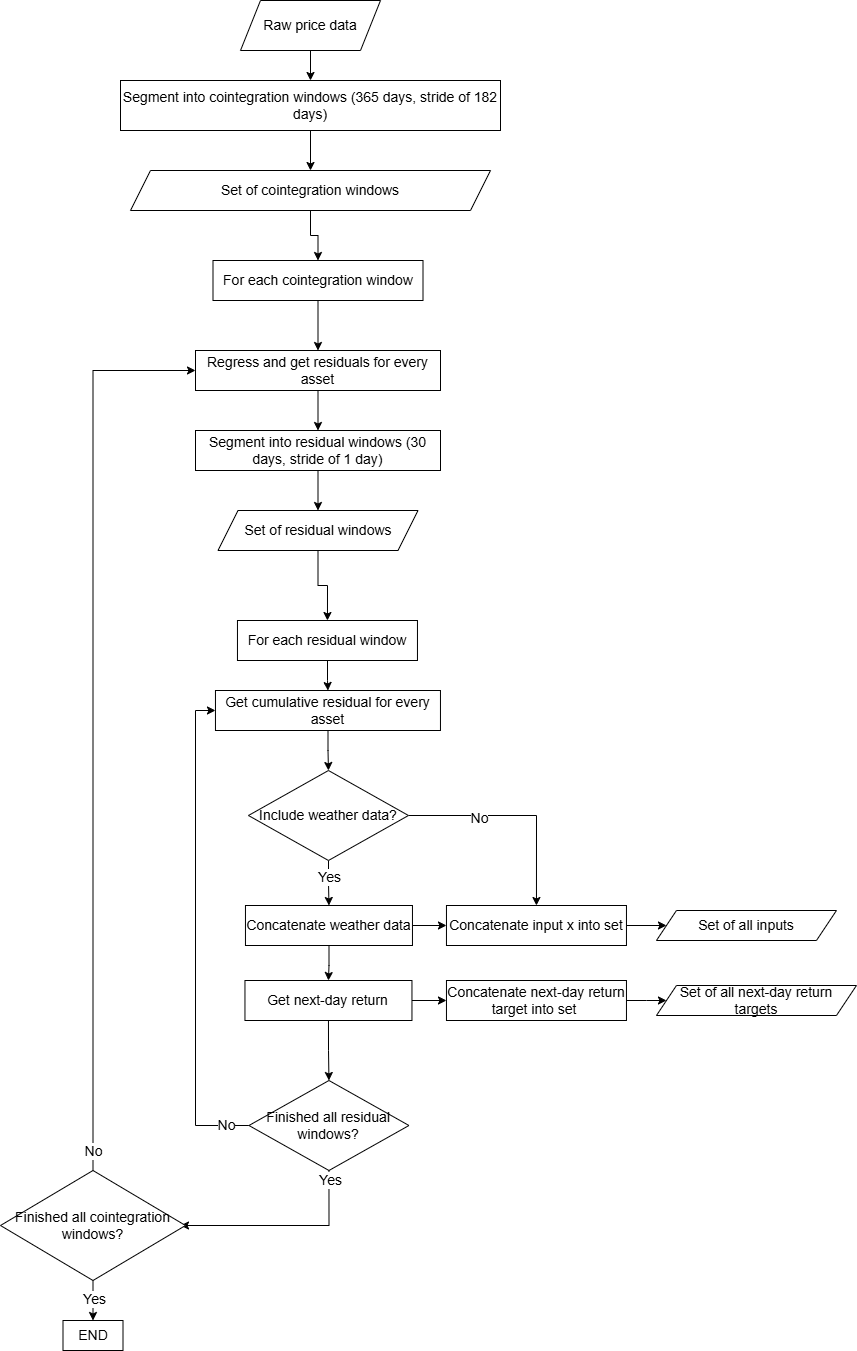
\includegraphics[width=0.8\textwidth]{assets/input_preparation_pipeline.drawio.png}
    \caption{Input Preparation Pipeline for Deep Learning Model}
    \label{fig:input_preparation_pipeline}
\end{figure}

% % Input figure of input preparation pipeline
% \begin{figure}[H]
%     \centering
%     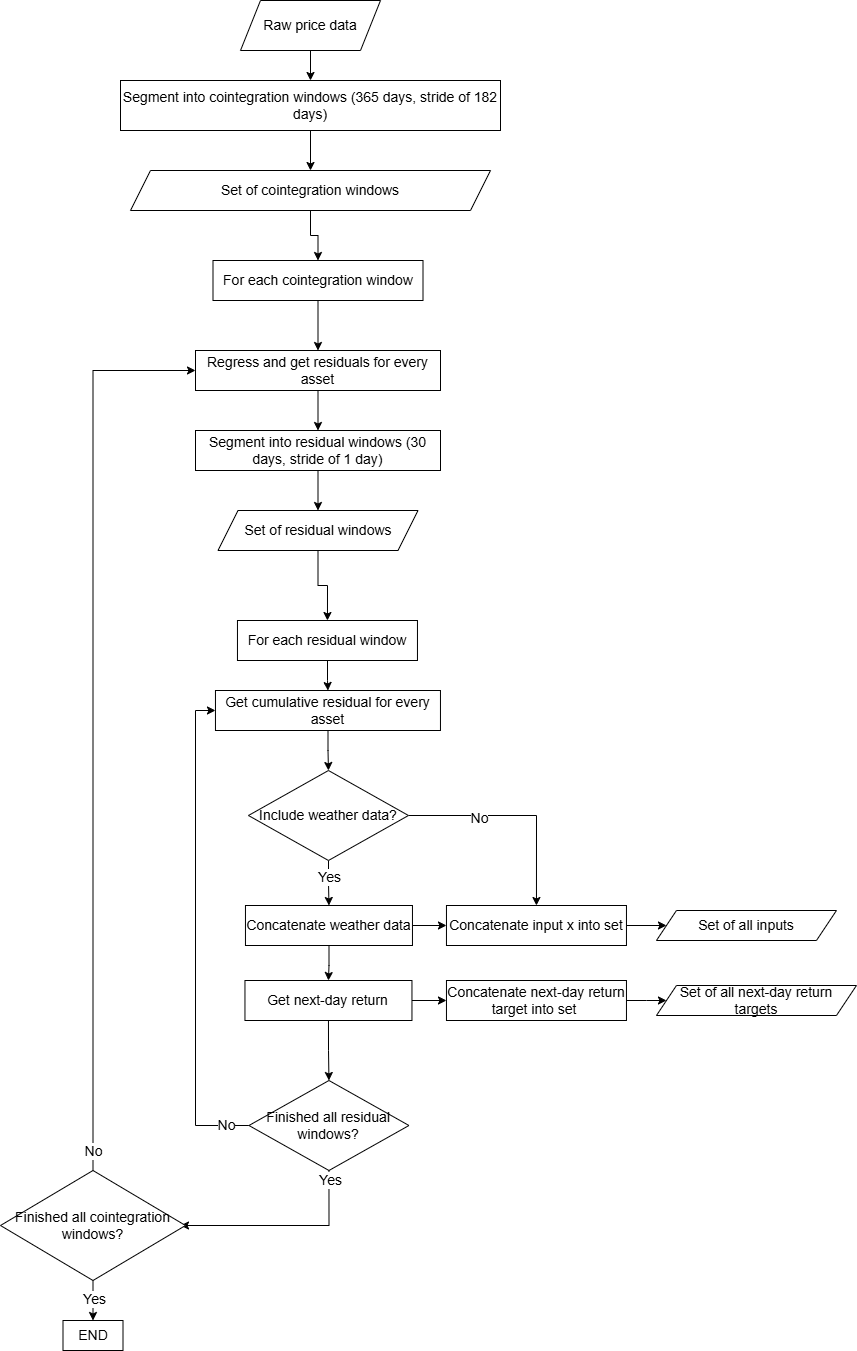
\includegraphics[width=0.8\textwidth]{assets/input_preparation_pipeline.drawio.png}
%     \caption{Input Preparation Pipeline for Deep Learning Model}
%     \label{fig:input_preparation_pipeline}
% \end{figure}

%Input pdf figure of data preparation pipeline
\begin{figure}[t]
    \centering
    \includegraphics[width=0.75\textwidth]{assets/input_preparation_pipeline_example1.pdf}
    \caption{Data Preparation Pipeline for Deep Learning Model (1 of 2, continued on next page)}
    \label{fig:data_preparation_pipeline1}
\end{figure}

\begin{figure}[t]
    \centering
    \includegraphics[width=0.6\textwidth]{assets/input_preparation_pipeline_example2.pdf}
    \caption{Data Preparation Pipeline for Deep Learning Model (2 of 2)}
    \label{fig:data_preparation_pipeline2}
\end{figure}


\begin{figure}
    \centering
    \begin{tikzpicture}[node distance=0.6cm and 0.5cm, scale=0.85, transform shape]
        % Top-level inputs
        \node[data] (price) {Price Matrix\\\texttt{(\#days,\#countries)}};
    
        
        
        \node[data, right=of price] (returns) {Returns\\\texttt{(\#(days-1),\#countries)}};
    
        \node[process, right=1.8cm of returns] (residuals) {Cointegration Residuals\\\texttt{(\#days,\#countries)}};
    
        % Preparation step
        \node[process, below=0.6cm of returns] (prep) {Rolling Window Prep\\Window Size = 30};

        \node[data, left=1cm of prep] (weather) {Weather Matrix\\\texttt{(\#days,\#countries*\#weather)}};
        
        % Combined final data
        \node[data, below=0.7cm of prep] (combined) {Combined Data\\\texttt{(\#days, \#features, window size)}};
    
        % Train/val/test split
        \node[process, below=0.8cm of combined] (split) {Train/Val/Test Split};
        \node[data, below left=0.6cm and 1.0cm of split] (train) {Train\\\texttt{(70\%)}};
        \node[data, below=0.6cm of split] (val) {Validation\\\texttt{(15\%)}};
        \node[data, below right=0.6cm and 1.0cm of split] (test) {Test\\\texttt{(15\%)}};
    I 
        % Arrows
        \draw[arrow] (price) -- (returns);
        \draw[arrow] (weather) -- (prep);
        \draw[arrow] (returns) -- (prep);
        \draw[arrow] (returns.east) to[out=0, in=90] (residuals.north);
        \draw[arrow] (residuals.south) to[out=-90, in=0] (prep.east);
    
        \draw[arrow] (prep) -- (combined);
        %\draw[arrow] (inputs.north) to[out=90, in=180] ([xshift=-0.8cm]combined.north);
        %\draw[arrow] (nextday.north) to[out=90, in=0] ([xshift=0.8cm]combined.north);
    
        \draw[arrow] (combined) -- (split);
        \draw[arrow] (split) -- (train);
        \draw[arrow] (split) -- (val);
        \draw[arrow] (split) -- (test);
    \end{tikzpicture}                     
    \caption{Data Processing Pipeline}
    \label{data_processing_pipeline}
\end{figure}

\begin{figure}
    \centering
    \begin{tikzpicture}[
      node distance=0.35cm,
      box/.style={draw, rounded corners, align=center, minimum height=1cm, minimum width=4cm, fill=blue!10},
      arrow/.style={-{Latex[width=2mm]}, thick}
    ]
    
    \node[box] (input) {Input\\{\tiny [Batch, Countries × Features, Time]}};
    \node[box, below=of input] (cnn) {CNN\\{\tiny Conv1D (filters=8, kernel=3) + ReLU + Flatten}};
    \node[box, below=of cnn] (transformer) {Transformer (optional) \\{\tiny 1 layer, 4 Attention Heads}};
    \node[box, below=of transformer] (ffn) {Feedforward NN\\{\tiny Hidden (8 if Transformer, else 64) → ReLU → Output}};
    \node[box, below=of ffn] (norm) {Soft Normalization\\{\tiny Tanh + Normalize (sum = 1)}};
    \node[box, below=of norm] (output) {Output Weights\\{\tiny [Batch, Countries]}};
    
    \draw[arrow] (input) -- (cnn);
    \draw[arrow] (cnn) -- (transformer);
    \draw[arrow] (transformer) -- (ffn);
    \draw[arrow] (ffn) -- (norm);
    \draw[arrow] (norm) -- (output);
    
    \end{tikzpicture}

    \caption{Model Architecture Overview}
    \label{model_architecture}
\end{figure}

\begin{figure}
\begin{tikzpicture}[node distance=1cm and 0.5cm, scale=0.95, transform shape]

    % Top Row: Input Data
    \node[data] (train_data) {Train + Val Data\\\texttt{(\#Days, \#Features, \#Window size)}};
    \node[data, right=6 cm of train_data] (test_data) {Test Data};

    % Middle Row: Training Stages
    \node[process, below=2cm of train_data] (grid_search) {Grid Search\\ filters=[8,16,32]\\size=[3,5,7]\\hidden=[64,128]};
    \node[process, right=of grid_search] (trainer) {Trainer\\ lr=0.00001, \\batch\_size=182, \\ patience=10000};
    \node[process, right=of trainer] (train_val) {Train on Train + Val\\Early Stopping};
    \node[process, right=of train_val] (test) {Test Evaluation\\Sharpe Ratio};

    % % Custom Loss Function (below Trainer)
    \node[loss, below right= 1 cm of trainer] (loss_fn) {Sharpe ratio loss: \\\texttt{$-\dfrac{R_t - R_f}{\sigma}$}};

    % % Custom Loss Function (below Trainer)
    \node[loss, below left= 1 cm of trainer] (optimizer) {Optimizer: \\\texttt{Adam}};

    % Arrows: Data Inputs
    \draw[arrow] (train_data) -- (grid_search);
    \draw[arrow] (test_data.south) -- (test.north);

    % Arrows: Process Flow
    \draw[arrow] (grid_search) -- (trainer);
    \draw[arrow] (trainer) -- (train_val);
    \draw[arrow] (train_val) -- (test);

    % Arrow: Trainer uses Custom Loss
    \draw[arrow] (loss_fn.north) -- (trainer.south);
    \draw[arrow] (optimizer.north) -- (trainer.south);
    
    \end{tikzpicture}
    \caption{Training and Evaluation}
    \label{training_and_evaluation}
\end{figure}